\begin{figure}[htbp]
  \centering
  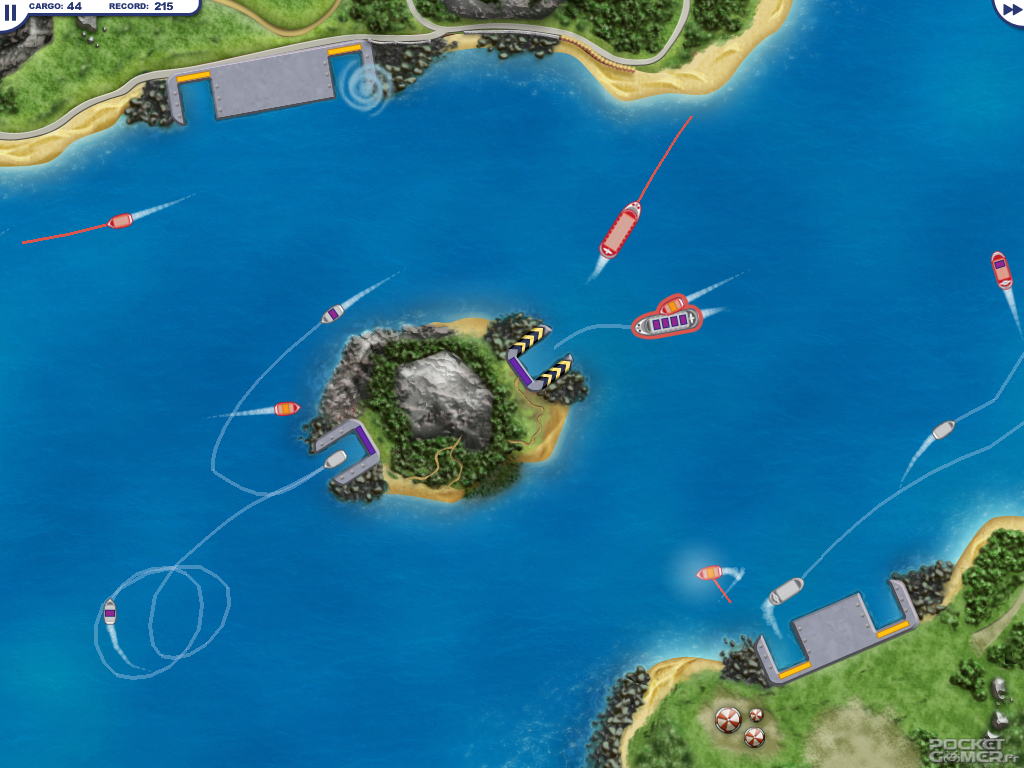
\includegraphics[width=\textwidth]{./images/harborMasterOriginal.png}
  \caption{Image du jeu original}
  \label{fig:harborMasterOriginal}
\end{figure}

Voilà comment se présente le jeu original (figure~\ref{fig:harborMasterOriginal}). N'ayant pas à nous attarder sur le graphisme du jeu, nous représenterons les bateaux par des formes simples selon leur type (carrés, cercles), et de même pour les ports. Une maquette est disponible en figure~\ref{fig:maquette}, l'aspect graphique définitif pourra différer. 


\begin{figure}[h]
	\begin{center}
		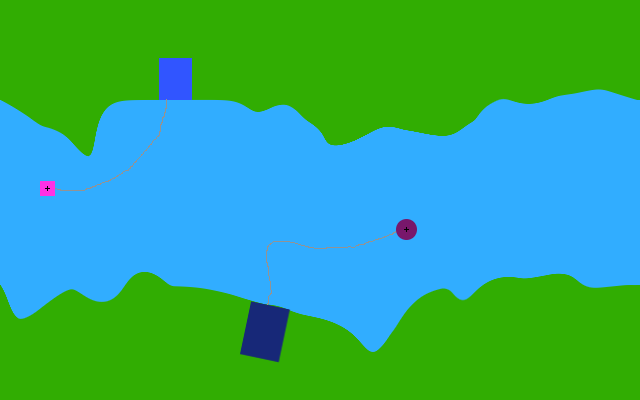
\includegraphics[width=\textwidth]{images/maquette}
	\end{center}
	\caption{Maquette de l'interface}
	\label{fig:maquette}
\end{figure}
